
%% bare_jrnl.tex
%% V1.4b
%% 2015/08/26
%% by Michael Shell
%% see http://www.michaelshell.org/
%% for current contact information.
%%
%% This is a skeleton file demonstrating the use of IEEEtran.cls
%% (requires IEEEtran.cls version 1.8b or later) with an IEEE
%% journal paper.
%%
%% Support sites:
%% http://www.michaelshell.org/tex/ieeetran/
%% http://www.ctan.org/pkg/ieeetran
%% and
%% http://www.ieee.org/

%%*************************************************************************
%% Legal Notice:
%% This code is offered as-is without any warranty either expressed or
%% implied; without even the implied warranty of MERCHANTABILITY or
%% FITNESS FOR A PARTICULAR PURPOSE! 
%% User assumes all risk.
%% In no event shall the IEEE or any contributor to this code be liable for
%% any damages or losses, including, but not limited to, incidental,
%% consequential, or any other damages, resulting from the use or misuse
%% of any information contained here.
%%
%% All comments are the opinions of their respective authors and are not
%% necessarily endorsed by the IEEE.
%%
%% This work is distributed under the LaTeX Project Public License (LPPL)
%% ( http://www.latex-project.org/ ) version 1.3, and may be freely used,
%% distributed and modified. A copy of the LPPL, version 1.3, is included
%% in the base LaTeX documentation of all distributions of LaTeX released
%% 2003/12/01 or later.
%% Retain all contribution notices and credits.
%% ** Modified files should be clearly indicated as such, including  **
%% ** renaming them and changing author support contact information. **
%%*************************************************************************


% *** Authors should verify (and, if needed, correct) their LaTeX system  ***
% *** with the testflow diagnostic prior to trusting their LaTeX platform ***
% *** with production work. The IEEE's font choices and paper sizes can   ***
% *** trigger bugs that do not appear when using other class files.       ***                          ***
% The testflow support page is at:
% http://www.michaelshell.org/tex/testflow/

% formatting instructions
% https://ras.papercept.net/conferences/support/files/IEEEtran_HOWTO.pdf

% from here
%https://journals.ieeeauthorcenter.ieee.org/create-your-ieee-journal-article/authoring-tools-and-templates/ieee-article-templates/templates-for-transactions/

\documentclass[journal]{IEEEtran}

\usepackage{cite}
\usepackage{amsmath}
\usepackage{url}
\usepackage{multirow}
% don't use the borders around links
\usepackage[hidelinks]{hyperref}

% *** GRAPHICS RELATED PACKAGES ***
%
\ifCLASSINFOpdf
\usepackage[pdftex]{graphicx}
% declare the path(s) where your graphic files are
\graphicspath{{../images/}}
% and their extensions so you won't have to specify these with
% every instance of \includegraphics
% \DeclareGraphicsExtensions{.pdf,.jpeg,.png}
\else
% or other class option (dvipsone, dvipdf, if not using dvips). graphicx
% will default to the driver specified in the system graphics.cfg if no
% driver is specified.
% \usepackage[dvips]{graphicx}
% declare the path(s) where your graphic files are
% \graphicspath{{../eps/}}
% and their extensions so you won't have to specify these with
% every instance of \includegraphics
% \DeclareGraphicsExtensions{.eps}
\fi

\begin{document}
	
	\title{Big Data Lake Solution for\\ 
		Warehousing Stock Data and Tweet Data}
	
	\author{Paul~Adams, paula@smu.edu,
		Rikel~Djoko, rdjoko@smu.edu,
		and Stuart Miller, stuart@smu.edu}% <-this % stops a space
	
	% The paper headers
	\markboth{MSDS7330 Term Paper Rough Draft}
	{MSDS7330 Term Paper Rough Draft}
	% The only time the second header will appear is for the odd numbered pages
	% after the title page when using the twoside option.
	
	% make the title area
	\maketitle
	
	% This should be about 250 words
	\begin{abstract}
		\textbf{Purpose} - This research paper aims to discover an optimal solution for parallel management and processing of financial markets data into  warehousing and analysis engines used for buy-sell decision-making. Methods analyzed herein are components of the Hadoop ecosystem. Included is an in-depth analysis of parallel processing - using the Elastic MapReduce package on Amazon Web Services - and data warehousing with Apache Hive. Apache NiFi is used to direct workflow automation for data migration into the warehouse. Finally, a complete assessment of the combinations of levels of the various Hadoop ecosystem applications used is provided in the context of statistical inference.
		
		\textbf{Design, Methodology, and Approach} - One pertinent, underlying hypothesis within this study is to prove that there are differences in processing speeds between S3 and HDFS using normalized and optimized schema designs across multiple MapReduce configurations. This analysis is performed using 100 samples of the same volume of data in a repeated measures analysis using a Hotelling-T statistic. The two highest-performing configurations of S3 and HDFS are then assessed. (We need to get this information and report it) for the next section.
		
		\textbf{Findings} - \textbf{EXAMPLE:} Applying S3 with an optimized schema using 10 reduces, map memory allocation of 2,048 mb and a reduce memory allocation of 4,096 mb is optimal for a more expensive S3 approach. Using HDFS from local storage with a configuration of 20 reduces, map memory allocation of 8,096 megabytes and reduce memory allocation of 10,020 megabytes is ideal for batch-level migrations and querying for large-volume processing. Across n repeated measures, using a one-tailed alpha, the resulting p-value is significant at `Pr > |t|` < x.xxxx (confidence interval (x1, x2)), indicating local storage from HDFS outperforms S3 when using the selected configurations. However, local data storage capacity does not scale well for HDFS compared to cloud-based S3.
	\end{abstract}
	
	% For peer review papers, you can put extra information on the cover
	% page as needed:
	% \ifCLASSOPTIONpeerreview
	% \begin{center} \bfseries EDICS Category: 3-BBND \end{center}
	% \fi
	%
	% For peerreview papers, this IEEEtran command inserts a page break and
	% creates the second title. It will be ignored for other modes.
	\IEEEpeerreviewmaketitle
	
	
	
	\section{Introduction}
	
	\IEEEPARstart{D}{ata} in the twenty-first century is expanding in volumes
	at exponential rates; every additional source of data that can act as a
	medium for data communication can obtain useful information, which,
	with modern technology, can be structured and stored, accessible to any
	who have the skills and need to make use of it \cite{BigDataComputing}. 
	This information is increasingly profitable. 
	However, with the increasing ability to capture and store data from many
	disparate sources, the need to store larger volumes of the data is
	likewise an increasing issue when it comes time to access and apply use,
	as many of the data gathered exist across very dynamic, diverse, and
	large partitions. 
	As such, the scalability of storing and accessing big data must increase
	with it, relevant to the structures and locations of these data repositories. 
	Developing a database in an ecosystem - Hadoop - that supports tools of
	two major concepts for achieving scalability within big data -
	data-parallelism and task-parallelism - our team has built a data
	warehousing solution to structure and store the data based on both
	optimized and normalized schema designs, drafted from entity-relationship
	models designed with the intention of enabling rapid storing and accessing
	through the Hadoop MapReduce process \cite{BigDataComputing}. 
	Through a combination of these systems and data storage within
	Amazon Simple Storage Service (S3) and Apache Hadoop's native Hadoop
	Distributed File System (HDFS), we analyze performance between two
	approaches toward data- and task-parallelism using data gathered from
	the stock market.
	
	\subsection{Apache Hadoop Ecosystem}
	
	Motivated through the opportunity within big data and parallel computing,
	which enables massive amounts of data to be rapidly accessed for complex
	analysis and distributed across a scalable, cost-effective distribution of
	servers. To accomplish this, we aligned our project with a modern database
	application called Hadoop. Hadoop provides a data lake ``ecosystem'' 
	supporting both task- and data-parallelism across the many software
	applications within the Apache suite in addition to software that can 
	be managed and accessed within a network of servers, called a cluster \cite{Intel, BigDataComputing}.
	
	The parallelism in Hadoop is categorized into data-parallelism and task-parallelism.
	Data-parallelism is focused on processing data across multiple processors whereas
	task-parallelism is focused on distributing execution threads across multiple servers \cite{Parallelism}. Utilizing one or the other is dependent upon whether data is 
	being provided into the system or being utilized for events such as machine learning.
	
	\subsection{Hadoop MapReduce}
	
	The server cluster enables users to read data from the same source,
	simultaneously, as the data at that source is partitioned and
	processed across multiple servers – a master and at least one slave. 
	The processing framework that enables this is called MapReduce, 
	which assigns nodes for ``mapping'' and ``reducing'' by applying 
	various configurations, such as related to memory allocation and numbers
	of mappers and reducers. As data is mapped, it is reprocessed into a derivative 
	data set, split into tuples that are then processed across the cluster, in parallel, and reassembled in the reduce process. Following the reduce process, data is delivered to 
	the end-user.
	
	\subsection{Application Integration and Data Ingestion}
	
	The parallelizability of Hadoop is central to this study as the primary
	objective is to rapidly store and access financial market data for 
	buy-sell decision-making. 
	The scope of applied analysis in this study is focused on the ability to
	scale and process a combination of quantitative stock market data and
	qualitative Twitter data related to the quantitative data. 
	
	Quantitative data was gathered from a markets data vendor through an
	Application Programming Interface (API) on 15-minute intervals using R
	programming language. 
	Qualitative data was gathered and processed through a Twitter API
	using Python programming language. 
	The data, structured and stored into a Hive data warehouse is created and
	managed using Hive Query Language (HQL) stored both locally and
	within an Amazon S3 storage bucket. 
	R will be used via Open Database Connectivity (ODBC) to access and
	build proof-of-concept models using the data. Once developed,
	Python will be deployed within the data lake to process and
	derive predictive data through machine learning decisions.
	
	\subsection{Big Data System Implementation}
	
	In order to provide manageable storage repositories that scale 
	well to size and data diversity, 
	we have implemented our solution using S3 and HDFS. 
	S3 and HDFS are designed for large sets of data. 
	Therefore, integrity of data and ingestion systems are able
	to be well maintained. 
	This is essential in an environment that may need to support 
	many simultaneous users, each with different data needs. 
	The HDFS implementation in this project is housed across three 
	- one master and two slave - Amazon EC2 servers 
	whereas S3 is a standalone repository within Amazon's cloud suite.
	
	Additionally, Apache Hive is used as a data warehouse 
	because it is operated with HQL, 
	which is easily communicable for SQL users. 
	Furthermore, Hive allows for storage of massive databases tables and
	is well-suited for big data application integration, 
	including the Apache software suite, of which Hadoop is a product. 
	The data warehouse graphical user interface is provided by Cloudera Hue.
	
	\subsection{Data Warehouse Schema and Selection}
	
	Two schemas were designed for the warehouse in a star configuration.
	This first schema was designed in a full normalized fashion,
	which is known as a snowflake schema.
	The second schema was based on the snowflake schema, 
	but denormalized to limit the number of tables, 
	which limits the number of joins required in queries.
	Query performance will be measured on these schemas to determine
	which design will be better for this use case. 
	
	
	\subsection{Performance Metrics and Evaluation}
	
	Performance is based on speed taken to process our 3 gigabytes of data 
	- once processed into their respective storage systems - 
	into the Hive data warehouse, which includes table creation and loading. 
	We will use a repeated measures analysis and a one-tailed hypothesis 
	test to determine optimal performance among S3 and HDFS groups, 
	which is then used to compare and assess benchmarks between the 
	combinations of MapReduce settings and database schemas among the
	best-performing S3 and HDFS configuration.
	
	
	
	
	\section{Data}
	
	This study investigates data warehouse models for housing stock
	price data and semi-structured alternative data. 
	Both daily and intraday stock price data were collected
	for use in this analysis. 
	Twitter was chosen as the primary source of alternative data because of
	ease-of-access to the \href{https://developer.twitter.com/en/docs}{Twitter API} 
	and the large volume of available data.
	The main features of the collected data are summarized in Table ~\ref{DataFeatures}.
	
	\begin{table}
		\renewcommand{\arraystretch}{1.3}
		\caption{Data Features}
		\label{DataFeatures}
		\centering
		\begin{tabular}{c|l}
			\hline
			Source       & Features\\
			\hline
			\hline
			Stock Daily  & Prices: High, Low, Open, Close\\
			\hline
			\multirow{10}{*}{Stock Intraday} &  Prices: High, Low, Open, Close \\
			&  High Bollinger bands\\
			&  Mid Bollinger bands\\
			&  Low Bollinger bands\\ 
			&  Nominal moving average\\
			&  Historical moving average\\
			&  Signal moving average\\ 
			&  Exponential moving average\\
			&  Stochastic 5-day indicator (Slow K)\\
			&  Stochastic 3-day indicator (Slow D)\\
			\hline
			Tweets       & Text, URLs, Hashtags, Mentions, Users\\
			\hline
		\end{tabular}
	\end{table}
	
	\subsection{Stock Data}
	
	The stock price data was collected through an API provided by
	\href{https://www.alphavantage.co/}{Alpha Vantage}.
	This API provided access to daily prices, intraday stock prices,
	and intraday price features.
	Intraday stock data contained 35 features sampled at 15 minute intervals. 
	The intraday features were from the following categories Bollinger bands, 
	stochastic oscillators, moving averages, and exponential moving averages.
	
	Approximately 1 million rows of data were collected,
	which occurred from Oct. 04, 2019 to Oct. 24, 2019.
	During the collection process, the data were recorded in files
	organized by day and category and stored in an S3 bucket.
	At the end of the collection process, the files for each
	category were combined and pushed to the HDFS datalake.
	
	\subsection{Twitter Data}
	
	Messages on Twitter (called tweets) are mainly comprised of
	tweet ID, timestamp, author (screen name), and text.
	Tweets can also contain many other features such as
	URLs, hashtags, emojis,  and mentions.
	For this analysis, in addition to the main features,
	URLs, hashtags, and mentions were also collected in the data warehouse.
	A mention is a reference to another Twitter user's screen name
	in the text of a tweet.
	A hashtag is some collection of characters starting with
	'\#' without white space.
	Generally, the character portion of a hashtag will be a word or set of words,
	but this is not necessary.
	
	Approximately 300,000 tweets were collected from over 100 Twitter users.
	The data from Twitter is returned in JavaScript Object Notation (JSON).
	The features of interest were extracted from the JSON files and
	reformatted in tab separated files (TSV).
	After the tweets were extracted from Twitter,
	mentions of company names or stock symbols were extracted from the tweet text by
	matching sections of tweet text to company names and company stock symbols.
	Once the data was collected and processed, it was pushed to the HDFS datalake.
	
	
	\section{Data Warehouse Development}
	
	Data warehouses are often conceptually designed with a \textit{star} schema 
	\cite{BuildingtheDWCH11}.
	In the star design, there is a central table (called the fact table),
	which contains the unifying features of the dataset and keys to other tables
	\cite{BuildingtheDWCH11}.
	The tables surrounding the fact table (called dimension tables) 
	contain information related to a category of the facts \cite{Enterprise}.
	In the dataset for this analysis, the unifying features are timestamp and
	company stock symbol, thus the fact table contains these features
	and several other descriptive features related to the companies.
	The natural dimensions of the fact table are intraday stock data,
	daily stock data, and tweet data.
	In some cases, dimensions of the facts exhibit an
	inherent hierarchical structure. 
	When the dimensions of a star schema are broken out into the tables
	that make up the hierarchical structure of the dimensions, the schema
	is in its \textit{snowflake} form \cite{WarehouseDesignApproaches}.
	In this study, two schemas were designed: one in snowflake form and
	the other in a more optimal form for query speed.
	
	\subsection{Snowflake Schema}
	
	\begin{figure}
		\centering
		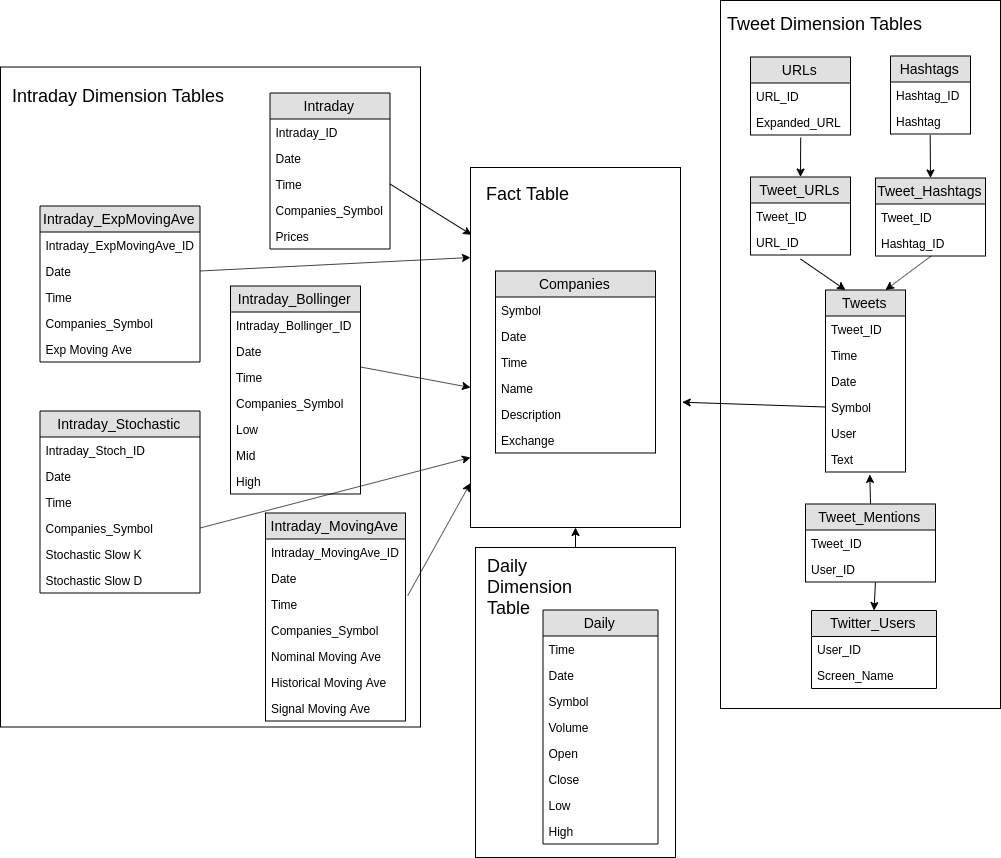
\includegraphics[width=2.5in]{Snowflake_Conceptual_Schema.png}
		\caption{Conceptual Diagram of the Data Warehouse Snowflake Schema}
		\label{snowflake}
	\end{figure}
	
	As noted previously, the fact table of this star design contained the
	company information and timestamps.
	The primary key of the fact table is a composite key that includes
	stock symbol and timestamp.
	There are three natural dimensions of fact table: daily stock data,
	intraday stock data, and tweet data.
	
	Both daily and intraday stock data are naturally keyed by the
	combination of timestamp and stock symbol,
	thus naturally keyed to the fact table.
	The stock data was spilt into two dimensions: daily data and intraday data.
	The daily data comes in a form suitable for the snowflake design.
	However, the intraday data was normalized into five tables for the 
	snowflake design: prices, Bollinger bands, moving averages, exponential
	moving averages, and stochastic indicators.
	The integration of the fact table and the normalized stock table is shown
	conceptually in Fig. \ref{snowflake} (left side of the schema diagram).
	
	Unlike the stock data, the tweet data did not naturally join to the fact
	table of the schema.
	Like the stock data, the tweet data came with a timestamp, but stock symbol
	is not a nominal feature of tweets.
	The stock symbol feature was generated by extracting matching strings
	during the data collection process; therefore, stock symbols are not
	guaranteed to be non-null in the tweet dimension.
	Additionally, the combination of timestamp and stock symbol is not guaranteed
	to be a primary key into the tweet table for tweets with non-null stock symbol
	fields.
	However, Twitter assigns a tweet ID for each tweet, which is guaranteed to be
	a primary key.
	Thus, the same features can still be used to join the tweet dimension to the 
	fact table, but cannot serve as a primary key.
	As noted previously, three secondary features of tweets are used in this study.
	Each of these features, mentions, hashtags, and URLs, represents a hierarchical
	member of the tweet dimension.
	Tables were created for each of these features to follow the snowflake design.
	These additional tables required join tables because there is a many-to-many
	cardinality between the tweet dimension and each of the three secondary members.
	The result of the tweet dimension normalization is shown conceptually
	in Fig. \ref{snowflake} (right side of schema diagram).
	
	\subsection{Denormalized Star Schema}
	
	While the snowflake schema is suitable for general use cases.
	The number of tables should be limited to decrease query time to support
	fast data transfer to a machine learning system.
	The number of intraday tables and tweet tables were reduced to support
	fast query times.
	All intraday tables were combined into one table. 
	Each secondary member of the Twitter dimension hierarchical structure was
	subsumed into a copy of the main tweet table, reducing the number of tables
	in the tweet dimension from seven to three.
	The schema resulting from this denomalization process is shown
	conceptually in Fig. \ref{star}.
	
	
	\begin{figure}
		\centering
		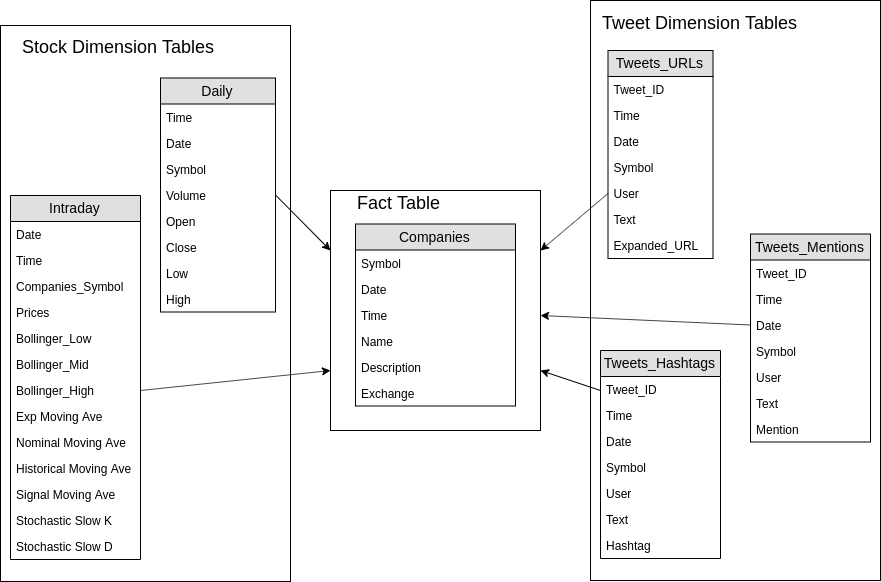
\includegraphics[width=2.5in]{Star_Conceptual_Schema.png}
		\caption{Conceptual Diagram of the Data Warehouse 
			Denormalized Star Schema}
		\label{star}
	\end{figure}
	
	\section{Implementation}
	
	Rikel
	
	\section{Results}
	
	Maybe a table comparing read times for the different options
	
	\begin{itemize}
		\item Snowflake vs Denormalized Star
		\item S3 vs HDFS
		\item HDFS mapreduce settings?
	\end{itemize}
	
	\section{Analysis}
	
	A statistical analysis of the results
	
	\begin{itemize}
		\item Discuss sample size of measures
		\item Looks like a repeated measures analysis
	\end{itemize}
	
	
	\section{Conclusion}
	\textbf{EXAMPLE CONCLUSION:}
	The scalability of large sets of data is of ever-increasing importance in the data community, which itself is ever-increasing with the advancement of modern technology. Modern technology itself is enabling both an increase in both data volume as well as data diversity being captured and stored. Consequently, parallelism is of utmost importance in making use of this data. Herein analyzed are methods that are proven within the scope of big data. As modern technology continues to advance, these parallel principals will serve as the root from which methodologies will be developed. As with the businesses and industries the data captured will serve, there will remain a trade-off that must be assessed for each business model. This study has provided two primary storage methods - S3 and HDFS - in addition to different data warehousing schema design - normalized versus optimized, star versus snowflake - and data distribution - herein, MapReduce - techniques. Through analysis using repeated measures, S3 outperforms HDFS when X, Y, Z and HDFS outperforms S3 when Z, Y, X. Furthermore, MapReduce configurations are constant across both storage methods - HDFS and S3 - with an optimized star schema performing faster, but a normalized snowflake schema performing more reliably within a conventional three-tiered system architecture.
	
	% Can use something like this to put references on a page
	% by themselves when using endfloat and the captionsoff option.
	\ifCLASSOPTIONcaptionsoff
	\newpage
	\fi
	
	\begin{thebibliography}{1}
		
		\bibitem{BigDataComputing}
		R. Kune, P. Konugurthi, A. Agarwal, R. Chillarige, R. Buyya,
		"The Anatomy of Big Data Computing," Software: Practice and Experience,
		Vol. 46 no. 1, pp.79-105, Jan. 2016. 
		
		\bibitem{BuildingtheDWCH11}
		W. H. Inmon, "Unstructured Data and the Data Warehouse," in 
		\emph{Building the Data Warehouse},
		4th ed. Hoboken: Wiley, 2005, ch. 11.
		Accessed on Nov. 6, 2019 [Online]. 
		Available: \\ https://learning.oreilly.com/library/view/building-the-data/9780764599446
		
		\bibitem{WarehouseDesignApproaches}
		I. Moalla, A. Nabli, L. Bouzguendam and M. Hammami,
		"Data warehouse design approaches from social media: review and comparison,"
		Social Network Analysis and Mining., Vol. 7, no. 1, pp. 1-14, Jan. 2017.
		Accessed on: Nov. 6, 2019 [Online]. 
		Available doi: 10.1007/s13278-017-0423-8
		
		\bibitem{Enterprise}
		A. Gorelik, "Historical Perspectives," in 
		\emph{The Enterprise Big Data Lake},
		1st ed. Sebastopol, CA: Wiley, 2019, ch. 2, pp. 25-47.
		
		\bibitem{Intel}
		"Extract, Transform, and Load Big Data with Apache Hadoop," Intel, USA, 2013.
		Available:\\ https://software.intel.com/sites/default/files/article/402274/etl-big-data-with-hadoop.pdf
		
		\bibitem{Parallelism}
		D. Sitaram, G. Manjunath \textit{Moving To The Cloud}. Boston: Syngress, 2012, pp. 205–253.
		
	\end{thebibliography}
	
	
	% that's all folks
\end{document}


